\documentclass[11pt]{article}

% ---------------------------------------------------------------------------
% Packages
% ---------------------------------------------------------------------------
\usepackage[margin=1in]{geometry}
\usepackage{amsmath,amssymb,amsthm}
\usepackage{booktabs}
\usepackage{graphicx}
\usepackage{xcolor}
\usepackage{hyperref}

\hypersetup{
  colorlinks = true,
  allcolors  = blue!60!black,
}

% ---------------------------------------------------------------------------
% Theorem environments
% ---------------------------------------------------------------------------
\newtheorem{theorem}{Theorem}[section]
\newtheorem{lemma}[theorem]{Lemma}
\newtheorem{proposition}[theorem]{Proposition}
\newtheorem{corollary}[theorem]{Corollary}
\theoremstyle{definition}
\newtheorem{definition}[theorem]{Definition}
\theoremstyle{remark}
\newtheorem{remark}[theorem]{Remark}

% ---------------------------------------------------------------------------
% Convenience macros
% ---------------------------------------------------------------------------
\newcommand{\RR}{\mathbb{R}}
\newcommand{\QQ}{\mathbb{Q}}
\newcommand{\energy}{E}
\newcommand{\pairP}{\operatorname{pairP}}
\newcommand{\triP}{\operatorname{triP}}
\newcommand{\BV}{\operatorname{BV}}

% Let the few long inline formulas break lines without overfull boxes.
\emergencystretch=2em

% ---------------------------------------------------------------------------
\title{Thomson Problem for $N=8$: Overview}
\author{Alexander Zughaid}
\date{\today}

\begin{document}

\maketitle

\section{Introduction}
\label{sec:introduction}

For $N$ distinct points $x_1,\dots,x_N$ on the unit sphere $S^2\subset\RR^3$,
the \emph{Thomson problem} asks for the configuration that minimises the
Coulomb energy
\begin{equation}
  \energy(x) \;=\; \sum_{i<j} \frac{1}{\lVert x_i - x_j\rVert}.
\end{equation}

The problem goes back to Thomson~\cite{Tho04}. Rigorous solutions are
known for only a few values of $N$.

For $N=8$, the square antiprism has long been the conjectured minimiser, proved rigorously by Kryvonos, Liehr, and Taylor~\cite{KLT26}. We
give a complete, machine-checked warrant of this fact in Lean~4, developed
with the assistance of generative AI. This document gives an overview of
the techniques used in that warrant.

\section{Method}
\label{sec:method}

\subsection{Statement: chords, inner products, and the energy}
\label{sec:method-statement}

\begin{definition}[Admissible]
A tuple $x=(x_1,\dots,x_8)\in(S^2)^8$ is \textbf{admissible} if
$\lVert x_i\rVert=1$ for every $i$, and $x_i\ne x_j$ whenever $i\ne j$.
\end{definition}

For an admissible $x$, write
\begin{equation}
  t_{ij} := \langle x_i, x_j \rangle, \qquad
  s_{ij} := \lVert x_i - x_j \rVert = \sqrt{2 - 2t_{ij}},
\end{equation}
for the inner product and \emph{chord length} of the pair $(i,j)$, so that
\begin{equation}
  \energy(x) \;=\; \sum_{i<j} \frac{1}{\sqrt{2-2t_{ij}}} \;=\; \sum_{i<j} \frac{1}{s_{ij}}.
\end{equation}

\subsection{The optimal antiprism height}
\label{sec:method-height}

Two squares of radius $r = \sqrt{1-h^2}$ at heights $\pm h$, offset by
$45^\circ$, form the \emph{antiprism} $\mathrm{antiprism}(h)$. Writing
$u = h^2$, $\alpha = 2-\sqrt2$, $\beta = 2+\sqrt2$, its energy has the closed
form (abusing notation, we write $\energy(u)$ for
$\energy(\mathrm{antiprism}(\sqrt u))$)
\begin{equation}
  \energy(u) \;=\; \frac{4\sqrt2+2}{\sqrt{1-u}} \;+\; \frac{8}{\sqrt{\alpha+\beta u}} \;+\; \frac{8}{\sqrt{\beta+\alpha u}}.
\end{equation}
Write $u^*$ for the minimiser of $\energy$ over this family:
\begin{equation}
  u^* = 0.3140893679\ldots, \qquad \energy(u^*) = 19.6752878612\ldots.
\end{equation}


\subsection{The four chord types and five triangle types}
\label{sec:method-chords}

At the optimal antiprism, the $\binom{8}{2}=28$ pairwise chords take only
four distinct values:

\begin{center}
\begin{tabular}{cll cc}
  \toprule
  label & geometric meaning & count & chord length & inner product \\
  \midrule
  $A$ & side of a square                        & 8 & $1.17125$ & $t_A = 0.31409$ \\
  $B$ & near cross-square pair                  & 8 & $1.28769$ & $t_B = 0.17092$ \\
  $C$ & diagonal of a square                     & 4 & $1.65639$ & $t_C = -0.37182$ \\
  $D$ & far cross-square pair                    & 8 & $1.89689$ & $t_D = -0.79910$ \\
  \bottomrule
\end{tabular}
\end{center}

Correspondingly, of the $\binom{8}{3}=56$ triangles $\{x_i,x_j,x_l\}$, only
five combinatorial types occur, written as their three chord labels in
decreasing order of length ($D>C>B>A$), occurring with multiplicities
\begin{equation}
  DDA\ (8), \quad DCB\ (16), \quad DBA\ (16), \quad CAA\ (8), \quad BBA\ (8).
\end{equation}

\begin{figure}[htbp]
\centering
\begin{minipage}{0.40\textwidth}
  \centering
  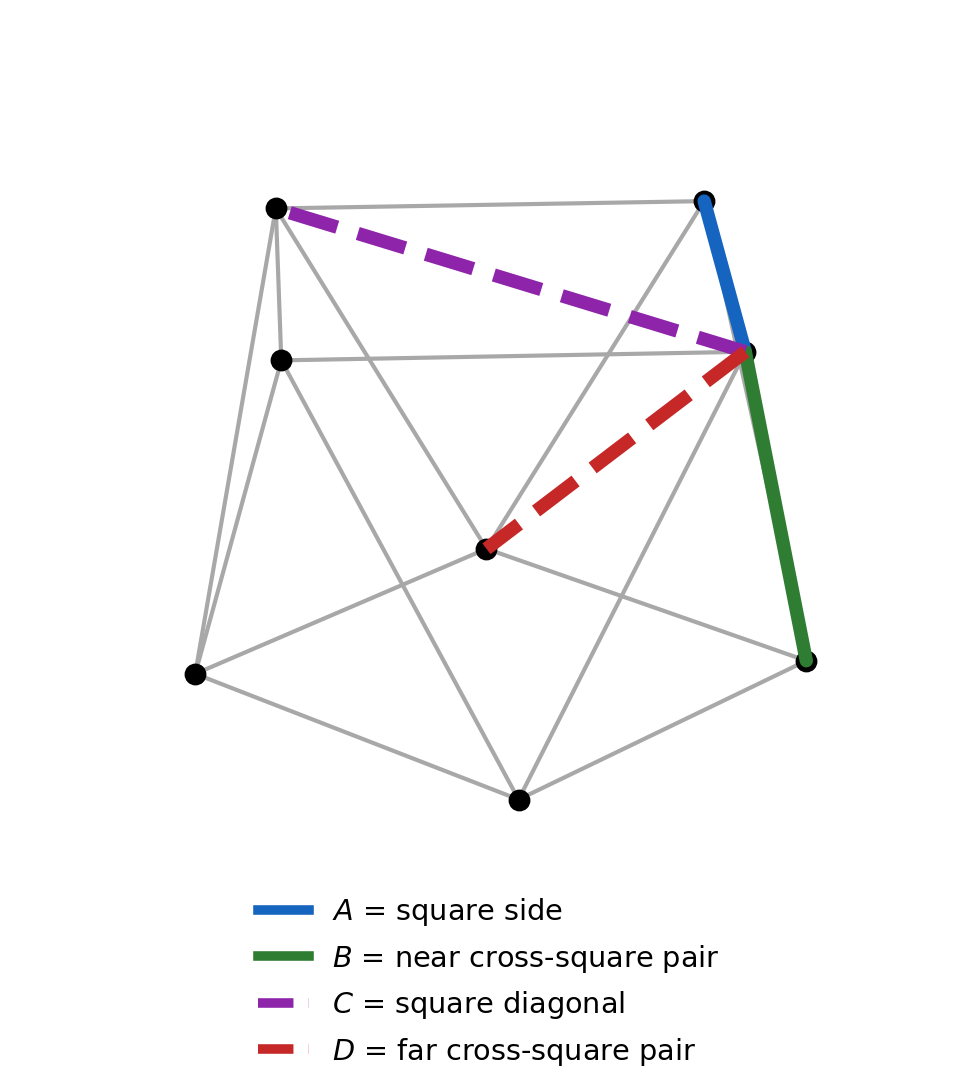
\includegraphics[width=\textwidth]{figures/chord_types_3d.png}
\end{minipage}
\hfill
\begin{minipage}{0.56\textwidth}
  \centering
  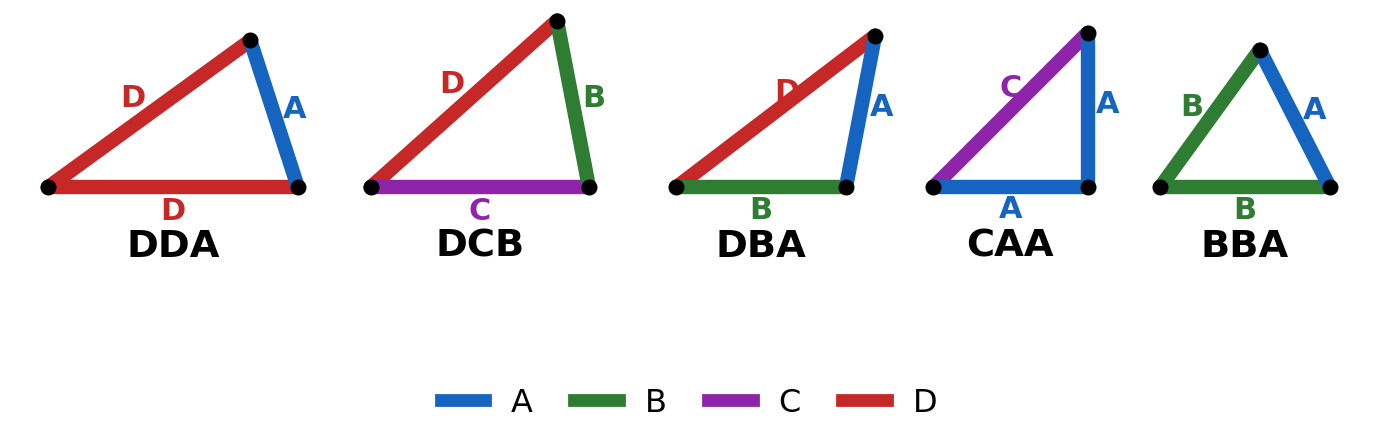
\includegraphics[width=\textwidth]{figures/triangle_types.png}
\end{minipage}
\caption{The antiprism, with one example edge of each chord type
highlighted and the five triangle types, drawn to scale, with sides coloured by
chord type.}
\label{fig:chords-triangles}
\end{figure}


\subsection{Bounding the chords: linear programming and the separation theorem}
\label{sec:method-separation}
The first step of the warrant is to put a \emph{lower} bound on each pairwise chord
length of a global minimum. Since $\energy(u^*) < 19.6753$, a global minimum $x$
satisfies $\energy(x) \le \energy(u^*) < 19.6753$.
Suppose we have a function $y$ of one chord length and a constant $b$ such that,
for every admissible $x$,
\begin{equation}
\label{eq:lp-hypotheses}
y(s_{ij}) \le \frac{1}{s_{ij}} \quad \text{for all } i \ne j,
\qquad
\sum_{i<j} y(s_{ij}) \;=\; b + \rho(x) \quad \text{with } \rho(x) \ge 0 .
\end{equation}
Adding and subtracting $y(s_{ij})$ in each term of the energy gives the identity
\begin{equation}
\label{eq:lp-identity}
\energy(x) \;=\; b \;+\; \sum_{i<j}\left(\frac{1}{s_{ij}} - y(s_{ij})\right) \;+\; \rho(x),
\end{equation}
in which every term after $b$ is nonnegative. Discarding all of them gives the
linear-programming bound $\energy(x)\ge b$; discarding all but one instead bounds
the \emph{slack} of a single pair by the excess of the energy over $b$,
\begin{equation}
\label{eq:lp-pair}
\frac{1}{s_{ij}} - y(s_{ij}) \;\le\; \energy(x) - b
\qquad \text{for all } i \ne j .
\end{equation}
For a global minimum, \eqref{eq:lp-pair} gives
$1/s_{ij} - y(s_{ij}) \le \varepsilon$ with $\varepsilon := 19.6753 - b$.
It is therefore enough to exhibit an $s_0$ with $1/s - y(s) > \varepsilon$ for
every $0 < s \le s_0$: no chord of a global minimum can then be at most $s_0$.
Multiplying by $s>0$, that is the positivity on $(0,s_0]$ of the one-variable
polynomial
\begin{equation}
\label{eq:lp-bernstein}
P(s) \;=\; 1 - s\,y(s) - \varepsilon s ,
\end{equation}
and positivity is certified by the positivity of all coefficients of
$P$ in the Bernstein basis of $[0,s_0]$.
Taking for $y$ Yudin's polynomial~\cite{Yud92} of degree $12$ in $t$, which touches $1/s$ at
three chord lengths and has $b = 19.6475639$, hence $\varepsilon = 0.0277361$, the polynomial $P$ has
degree 25 and all $26$ of its Bernstein coefficients on $[0,0.962]$ are
positive. This two-point linear-programming argument~\cite{DGS77,Yud92}, applied to
the near-optimal region, is the \textbf{separation theorem}:
\begin{equation}
\label{eq:separation}
\energy(x) \le 19.6753 \quad\Longrightarrow\quad s_{ij} > 0.962 \ \text{ for all } i\ne j,
\end{equation}
equivalently $t_{ij} < 0.53728$. Below, these are used in the slightly
weaker, rounder forms $t_{ij}\le0.5373$ and $s_{ij}\in[0.9619,2]$. Any
configuration that could match or beat the antiprism therefore has all of
its chords in this range.



\subsection{Defining the data structure}
\label{sec:method-bv}
\label{sec:method-datum}

\paragraph{The Bachoc--Vallentin matrices.}
Bachoc and Vallentin~\cite{BV08} introduced three-point semidefinite
bounds for spherical codes, built from a matrix kernel $S_k^n(u,v,t)$,
symmetrised from a Chebyshev/Gegenbauer kernel so that
$\sum S_k^n\succeq0$ automatically over any finite point set on
$S^{n-1}$; Cohn and Woo~\cite{CW12} adapted these bounds to energy
minimisation. For $S^2$, truncated at degree $d$ ($k\le d$ and
$i,j\le d-k$; here $d=8$, giving $(9-k)\times(9-k)$ blocks), with $T_k$
the degree-$k$ Chebyshev polynomial (here $u,v,t$ denote generic inner
products, unrelated to the antiprism parameter $u=h^2$):
\begin{equation}
  Y_k(u,v,t)_{ij} \;=\; u^i v^j \big((1-u^2)(1-v^2)\big)^{k/2}\, T_k\!\left(\frac{t-uv}{\sqrt{(1-u^2)(1-v^2)}}\right),
\end{equation}
\begin{equation}
  S_k(u,v,t) \;=\; \frac16 \sum_{\sigma \in S_3} Y_k(u,v,t)\circ\sigma.
\end{equation}

The classical two-point method of Delsarte, Goethals and
Seidel~\cite{DGS77}, in Yudin's energy version~\cite{Yud92}, used in
\S\ref{sec:method-separation}, bounds each pair separately, and for
$N=8$ this is not enough: Yudin's degree-$12$ polynomial gives
$b=19.6475639$, short of $\energy(u^*)=19.675288\ldots$ by $0.0277$, and
no choice of $y$ does better than about $19.6478$.
The three-point method below applies the same argument to triangles as
well as pairs.

The energy can be written in two ways. As a sum over pairs, by
definition,
\begin{equation}
  \label{eq:energy-pairs}
  \energy(x) \;=\; \sum_{i<j} \frac{1}{s_{ij}},
\end{equation}
and, since every pair $\{i,j\}$ lies in exactly $6$ of the $56$
triangles, as a sum over triangles,
\begin{equation}
  \label{eq:energy-triangles}
  \energy(x) \;=\; \frac16\sum_{i<j<l}\left(\frac1{s_{ij}}+\frac1{s_{il}}+\frac1{s_{jl}}\right).
\end{equation}
Taking $1-18\lambda$ times \eqref{eq:energy-pairs} plus $18\lambda$
times \eqref{eq:energy-triangles} splits the energy between the two,
for any real $\lambda$:
\begin{equation}
  \label{eq:lambda-split}
  \energy(x) \;=\; \underbrace{\sum_{i<j} (1-18\lambda)\frac{1}{s_{ij}}}_{\text{a sum over pairs}}
  \;+\; \underbrace{3\lambda \sum_{i<j<l}\left(\frac1{s_{ij}}+\frac1{s_{il}}+\frac1{s_{jl}}\right)}_{\text{a sum over triangles}}.
\end{equation}
The two sums are bounded by different methods, so the bound obtained
depends on $\lambda$, which is a free parameter of the certificate. At $\lambda=0$ the triangle sum
drops out and the classical sum over pairs remains.

\paragraph{Bounding each sum.} Each of the two sums is treated the way
the classical method treats a sum over pairs: from each term, subtract a
function of that term alone, chosen so that every difference (a
\emph{slack}) is nonnegative and the sum of the subtracted functions is
bounded below by a constant independent of the configuration.

For the pairs, subtract a function $L$ of the pair's inner product. It
must lie below the pair's share, and $\sum_{i<j}L(t_{ij})$ must be
bounded below whatever the configuration. Schoenberg's
theorem~\cite{Sch42} gives
the second requirement, as for the two-point method above, and
so dictates the form of $L$: written in the Legendre basis, its
coefficients in degrees $1$ and above must be nonnegative. In this work
$L$ is taken to be linear, $L(t)=a_0+a_1t$, so the only condition is
$a_1\ge0$.

For the triangles, subtract a function $K$ of the triangle's three
inner products. It must lie below the triangle's share, and
$\sum_{i<j<l}K$ must be bounded below whatever the configuration. This
is the new ingredient, and the reason the method is called three-point:
a pair-based bound never uses the fact that the chords come from points
of $\RR^3$, whereas the three inner products of a triangle are
constrained, since three unit vectors of $\RR^3$ cannot meet at
arbitrary angles. Bachoc and Vallentin supply the required bound. Their
positivity statement is about a matrix rather than a number, so the
corresponding free parameter is a positive semidefinite matrix, one for
each degree: $K_0,\dots,K_5$ here.

The Bachoc--Vallentin sum runs over \emph{all} ordered triples of
points, including degenerate ones in which two of the points coincide.
Such a triple has inner products $(1,t,t)$, where $t$ is the inner
product of the remaining pair, so its term is a function of that pair
alone and belongs with the pair sum. What is subtracted from each pair's
share is therefore not $L(t)$ alone but $L(t)+3K(1,t,t)$, the factor $3$
counting the three positions the repeated point can occupy in an
ordered triple; the fully degenerate triples, with inner products
$(1,1,1)$, contribute only a constant, which goes into the bound
(\S\ref{sec:method-identity}).

A \textbf{data structure} packages $L$, $\lambda$, and the matrices
$K_0,\ldots,K_5$ into one tuple:
\begin{equation}
  \mathcal{D} \;=\; (a_0,\, a_1,\, \lambda,\, K_0,\, K_1,\, K_2,\, K_3,\, K_4,\, K_5).
\end{equation}
Its entries are as follows.

\begin{description}
\item[$a_0,a_1\in\RR$ (classical).] The coefficients of the
  \textbf{linear potential}
  \begin{equation}
    L(t) \;:=\; a_0 + a_1 t.
  \end{equation}
  Writing $\mu(x):=\sum_i\sum_j t_{ij}=\lVert\sum_i x_i\rVert^2$, the
  side condition is $a_1\ge0$; the resulting \textbf{design term}
  $a_1\mu(x)$ vanishes at any antiprism, since
  its eight points always sum to $\mathbf{0}$ by symmetry.

\item[$\lambda\in\RR$, $0\le\lambda\le\tfrac1{18}$.] The
  scalar governing the pair/triangle split in \eqref{eq:lambda-split},
  which combines the two separate Bachoc--Vallentin constraints into a
  single bound. For $N=8$, taking $\lambda=0$ gives at
  best $\approx19.6730$, short of $\energy(u^*)$ even with the matrices
  $K_0,\ldots,K_5$, so a positive $\lambda$ is needed.

\item[$K_0,\dots,K_5$ \cite{BV08,CW12}.] The Bachoc--Vallentin
  matrix variables, six of them as in the example of Cohn and Woo: positive
  semidefinite matrices of sizes $9,8,7,6,5,4$ respectively. For $N=8$,
  the blocks $K_6,K_7,K_8$ allowed by the degree-$8$ truncation are zero
  in the optimal certificate and are omitted; truncating at degree $4$ or
  $6$ instead gives a valid bound that falls short of $\energy(u^*)$ by
  $0.023$ and $0.006$ respectively. With the Bachoc--Vallentin matrices
  $S_k(u,v,t)$ above, these assemble into the \textbf{kernel function}
  \begin{equation}
    K(u,v,t) \;:=\; \sum_{k=0}^{5} \langle K_k,\, S_k(u,v,t) \rangle.
  \end{equation}
\end{description}

From here on, $\mathcal{D}$ denotes an arbitrary data structure and
$\mathcal{D}^*$ the specific one constructed in
\S\ref{sec:method-pivots}.

\subsection{The bound-plus-slack identity}
\label{sec:method-terms}
\label{sec:method-identity}

The analogue of the two-point identity~\eqref{eq:lp-identity} has two
kinds of slack term instead of one. The two Bachoc--Vallentin constraints
are both built from the same three-point kernel $K$: one evaluated at a
repeated triple $(t,t,1)$, which collapses two of the three points
together and so is a statement about pairs; the other at the inner
products $(u,v,w)$ of three distinct points, a statement about
triangles. In the present notation these give pairSlack and triSlack
respectively, their matrix positivity gives $\BV$, and $a_1\ge0$ gives
the design term:
\begin{align}
  \BV(x) &:= \sum_{i,j,l=1}^{8} K(t_{ij},t_{il},t_{jl}), \\
  \mathrm{pairSlack}(\mathcal{D},x,i,j) &:= (1-18\lambda)\frac{1}{s_{ij}} - a_0 - a_1 t_{ij} - 3K(1,t_{ij},t_{ij}), \\
  \mathrm{triSlack}(\mathcal{D},x,i,j,l) &:= \lambda\left(\frac1{s_{ij}}+\frac1{s_{il}}+\frac1{s_{jl}}\right) - K(t_{ij},t_{il},t_{jl}), \\
  \text{design term} &:= a_1 \mu(x).
\end{align}
Adding and subtracting these same quantities in every pairwise and
triangle term of the energy, the way $y(s_{ij})$ was added and
subtracted for the two-point bound, and summing over the $28$ pairs and
$56$ triangles, collects them into the single quantity
\begin{equation}
  2f(\mathcal{D},x) \;:=\; \BV(x) \;+\; 2\sum_{i<j}\mathrm{pairSlack}(\mathcal{D},x,i,j)
  \;+\; 6\sum_{i<j<l}\mathrm{triSlack}(\mathcal{D},x,i,j,l) \;+\; a_1\mu(x),
\end{equation}
the factors $2$ and $6$ counting each pair and each triangle once for
every ordering of its indices, since $\mathrm{pairSlack}$ and
$\mathrm{triSlack}$ depend only on the unordered pair or triangle.
With $L$ as above, setting the \textbf{bound}
\begin{equation}
  b(\mathcal{D}) \;:=\; \frac{64a_0 - 8L(1) - 8K(1,1,1)}{2} \;=\; 28a_0 - 4a_1 - 4K(1,1,1),
\end{equation}
to collect the leftover constant terms gives, for every admissible $x$
and every data structure, the exact identity (Bachoc and Vallentin~\cite{BV08} and Cohn and
Woo~\cite{CW12} state only the inequality it implies)
\begin{equation}
  \label{eq:main-identity}
  \energy(x) \;=\; b(\mathcal{D}) \;+\; f(\mathcal{D},x).
\end{equation}
As with the two-point bound, if $f(\mathcal{D},x)\ge0$ then
$\energy(x)\ge b(\mathcal{D})$. The rest of this section constructs a data
structure with $b(\mathcal{D})=\energy(u^*)$ and $f(\mathcal{D},x)\ge0$
for every $x$ satisfying the separation bound~\eqref{eq:separation}.

\subsection{The polynomials \texorpdfstring{$\pairP$}{pairP} and \texorpdfstring{$\triP$}{triP}}
\label{sec:method-nonneg}
\label{sec:method-pairP-triP}

Two of the four terms are automatically nonnegative for every admissible
$x$: $\BV$ from $K_k\succeq0$, and the design term from $a_1\ge0$. The
other two, pairSlack and triSlack, need the two Bachoc--Vallentin
constraints, specialised to this problem. Clearing denominators in
$\mathrm{pairSlack}\ge0$ and $\mathrm{triSlack}\ge0$ turns each into a
polynomial inequality:
\begin{equation}
  \pairP(\mathcal{D},s) \;:=\; (1-18\lambda) \;-\; s\Big[a_0 + a_1\big(1-\tfrac{s^2}2\big) + 3K\big(1,\,1-\tfrac{s^2}2,\,1-\tfrac{s^2}2\big)\Big],
\end{equation}
\begin{equation}
  \triP(\mathcal{D},p,q,r) \;:=\; \lambda(qr+pr+pq) \;-\; pqr\cdot K\big(1-\tfrac{p^2}2,\,1-\tfrac{q^2}2,\,1-\tfrac{r^2}2\big),
\end{equation}
with $\mathrm{pairSlack} = \pairP(\mathcal{D},s_{ij})/s_{ij}$ and
$\mathrm{triSlack} = \triP(\mathcal{D},p,q,r)/(pqr)$, so $f(\mathcal{D},x)\ge0$
follows once $\pairP(\mathcal{D},\cdot)\ge0$ and
$\triP(\mathcal{D},\cdot,\cdot,\cdot)\ge0$ hold on the relevant ranges.

As with the two-point bound, a plain inequality is not enough to make
the bound sharp: following Yudin, what is needed is a double zero at
the target configuration. At the
certificate $\mathcal{D}^*$, $\pairP(\mathcal{D}^*,\cdot)$ has a double zero at each of the
four chords $A,B,C,D$, and $\triP(\mathcal{D}^*,\cdot,\cdot,\cdot)$ vanishes
(value and gradient) at each of the five triangle types, pinning
$\mathcal{D}^*$'s $24$ free entries down to specific numbers, via the linear
system built next.

\subsection{Constructing \texorpdfstring{$\mathcal{D}^*$}{D*}: the pivot system and the \texorpdfstring{$24\times24$}{24x24} matrix \texorpdfstring{$M$}{M}}
\label{sec:method-pivots}

The identity~\eqref{eq:main-identity} holds for every data structure,
but for a generic one the resulting bound is not sharp:
$b(\mathcal{D})<\energy(u^*)$. The data structure $\mathcal{D}^*$ is
therefore constructed with $b(\mathcal{D}^*)=\energy(u^*)$ as one of its
defining equations.

The six blocks $K_0,\ldots,K_5$ have $45+36+28+21+15+10=155$ independent
entries. Two reductions bring the number of unknowns down to $24$.

First, equality at the antiprism forces $\BV(\mathrm{antiprism})=0$. Summed
over the antiprism, $\sum_{i,j,l}S_k(t_{ij},t_{il},t_{jl})$ has rank one,
say $v_kv_k^\top$, so for $K_k\succeq0$ this is complementary slackness,
$K_kv_k=0$. Each block is therefore written as
$K_k = B_k H_k' B_k^\top$, where the columns of the fixed basis matrix
$B_k$ span $v_k^\perp$ (its entries are polynomials in $u^*$ with
rational coefficients). This builds $K_kv_k=0$ in, absorbing $39$ linear
constraints and leaving $36+28+21+15+10+6=116$ free entries across the
$H_k'$. Together with $a_0,a_1,\lambda$ that makes $119$ numbers.

Second, $95$ of these (namely $a_0,a_1,\lambda$ and $92$ entries of the
$H_k'$) are fixed explicit rationals. The remaining $24$, the
\textbf{pivots}, are determined by $24$ linear tightness conditions:

\begin{center}
\begin{tabular}{cl}
  \toprule
  rows & condition \\
  \midrule
  $1$  & $b(\mathcal{D}^*) = \energy(u^*)$ \\
  $3$  & $\pairP(\mathcal{D}^*,s_X) = 0$ for $X \in \{B,C,D\}$ \\
  $4$  & $\pairP'(\mathcal{D}^*,s_X) = 0$ for all four chords $X \in \{A,B,C,D\}$ \\
  $5$  & $\triP(\mathcal{D}^*,\cdot) = 0$ at each of the five triangle types \\
  $11$ & gradient components of $\triP(\mathcal{D}^*,\cdot)$ at the five types (all but one) \\
  \bottomrule
\end{tabular}
\end{center}

Full tightness asks for $26$ conditions: the bound, a value and a
derivative of $\pairP$ at each of the four chords, and a value and the
gradient of $\triP$ at each of the five triangle types. Since $\triP$ is
symmetric in its three arguments, a type with a repeated chord has only
two distinct gradient components, so the gradients contribute
$2+3+3+2+2=12$ conditions. The $26$ conditions have rank $24$, and two are
dropped. The value $\pairP(\mathcal{D}^*,s_A)=0$ is dropped because it follows
from the others. Evaluating the identity~\eqref{eq:main-identity} at the
antiprism, where $\BV=0$ (built in via $K_kv_k=0$ below) and $\mu=0$,
gives the affine relation
\begin{equation}
  \energy(u^*) - b(\mathcal{D}) \;=\; \sum_{X} n_X\,\frac{\pairP(\mathcal{D},s_X)}{s_X}
  \;+\; 3\sum_{T} m_T\,\frac{\triP(\mathcal{D},T)}{p_Tq_Tr_T},
\end{equation}
where $X$ runs over the four chords with counts $n_X$, and $T=(p_T,q_T,r_T)$
over the five triangle types with multiplicities $m_T$. Once the bound
row and the other eight value rows hold, only the term $n_A\,\pairP(\mathcal{D},s_A)/s_A$
remains, and $n_A=8\ne0$ forces it to vanish. One gradient component
at the type $DCB$ is dropped because it follows from
$\energy'(u^*)=0$, by differentiating the identity~\eqref{eq:main-identity}
along the antiprism family. Both dropped conditions are proved in Lean to
hold once $M$ below is invertible. The remaining rows sum to
$1+3+4+5+11=24$, exactly the number of pivots, so the system is square.
Since $b(\mathcal{D})$, $\pairP(\mathcal{D},\cdot)$, and
$\triP(\mathcal{D},\cdot)$ are each affine in the pivots once the chord and
triangle inputs are fixed, these 24 conditions assemble into a linear
system in the pivot vector $\mathbf{p}\in\RR^{24}$, and the pivots are
\emph{defined} as its solution:
\begin{equation}
  M\mathbf{p} \;=\; \mathbf{c}, \qquad
  \mathbf{p}^* \;:=\; M^{-1}\mathbf{c}
\end{equation}
(\texttt{pivotMatrix}, \texttt{pivotRhs} and \texttt{pivots} in the Lean
code).
If $M$ is invertible, all $24$ tightness conditions hold at
$\mathbf{p}^*$ by construction. The
$24\times24$ matrix $M$ and the vector $\mathbf{c}\in\RR^{24}$ are built
from the fixed entries, the bases $B_k$, and the chord and triangle data,
so, like $u^*$ itself, they are irrational. $\mathcal{D}^*$ is the data
structure with the fixed rational entries and the exact pivots $\mathbf{p}^*$.

\paragraph{Why the certificate is implicit.} Exact tightness places the
pivots in the degree-$192$ number field generated by $\sqrt2$, $u^*$ and
the chord lengths, where their coefficients have about $15\,000$ digits;
a data structure with rational entries could prove at best
$\energy(x)\ge\energy(u^*)-\varepsilon$ for some $\varepsilon>0$. The
warrant therefore keeps $\mathcal{D}^*$ implicit and works with an explicit
$22$-digit rational vector
$\tilde{\mathbf{p}}\in\QQ^{24}$ (\texttt{pivotsNum} in the Lean code)
and a proved enclosure of $\mathbf{p}^*$
around it (fact~(i) below). Everything built from $\mathcal{D}^*$ is affine
in the pivots, so an inequality checked at $\tilde{\mathbf{p}}$ with a
positive margin transfers to $\mathcal{D}^*$, with an explicit error
bound. All numerical checking is therefore done in rational interval
arithmetic, while the tightness conditions hold exactly.

\subsection{The properties of \texorpdfstring{$\mathcal{D}^*$}{D*}}
\label{sec:method-four-facts}

\begin{definition}[Realisable triangle region]
A triple $(p,q,r)\in[0.9619,2]^3$ lies in the \textbf{realisable triangle
region} if, writing $u=1-\tfrac{p^2}2,\ v=1-\tfrac{q^2}2,\ w=1-\tfrac{r^2}2$
for the corresponding inner products, the Gram matrix
$\left(\begin{smallmatrix}1&u&v\\ u&1&w\\ v&w&1\end{smallmatrix}\right)$ is
positive semidefinite, equivalently
\begin{equation}
  1 + 2uvw - u^2 - v^2 - w^2 \;\ge\; 0.
\end{equation}
This is exactly the condition for $(p,q,r)$ to be realisable as the three
chord lengths of an actual spherical triangle $\{x_i,x_j,x_l\}\subset S^2$.
\end{definition}

The warrant needs four facts about $\mathcal{D}^*$. Fact (ii) gives
$\BV(x)\ge0$; facts (iii) and (iv) give $\pairP(\mathcal{D}^*,\cdot)\ge0$
and $\triP(\mathcal{D}^*,\cdot,\cdot,\cdot)\ge0$; fact (i) makes
$\mathcal{D}^*$ well defined and allows the other three to be checked at
the rational vector $\tilde{\mathbf{p}}$ instead of the irrational $\mathbf{p}^*$.

\begin{enumerate}
  \item[(i)] The matrix $M$ is invertible, and
    $\lVert\mathbf{p}^*-\tilde{\mathbf{p}}\rVert_\infty\le2\times10^{-21}$. (Facts (ii)--(iv) need only $10^{-12}$.)
  \item[(ii)] Each block $H_k'$, and hence each $K_k=B_kH_k'B_k^\top$, is
    positive semidefinite.
  \item[(iii)] We have $\pairP(\mathcal{D}^*,\cdot)\ge0$ on $[0.9619,2]$.
  \item[(iv)] We have $\triP(\mathcal{D}^*,\cdot,\cdot,\cdot)\ge0$ on the realisable
    triangle region.
\end{enumerate}

\subsection{Verifying the properties using the Lean kernel}
\label{sec:method-verification}

Facts (i)--(iv) are proved by reflection. For each fact, a Lean checker
evaluates the relevant polynomials in fixed-point interval arithmetic on
rational data (the fixed entries, $\tilde{\mathbf{p}}$, and rational
enclosures of $u^*$ and the chord lengths), and a soundness theorem
transfers its output to the real statement. The checkers are evaluated
in the kernel with \texttt{decide +kernel}, so the warrant uses only Lean's
three standard axioms; the largest check, part of fact (iv), takes about
30 CPU-hours.

Facts (ii)--(iv) are checked at $\tilde{\mathbf{p}}$ with a positive
margin. Since everything is affine in the pivots, fact (i) bounds the
change in moving to $\mathbf{p}^*$ by $10^{-12}$ times an explicit
rational $\ell^1$-norm, which the margin absorbs. Facts (iii) and (iv)
are checked by subdividing their domains into boxes. At the four chords
and five triangle types, where $\pairP$ and $\triP$ vanish, a certified
quadratic lower bound is used instead, and the perturbation bound is
applied only after these zeros have been divided out.

The fixed entries and $\tilde{\mathbf{p}}$ come from a floating-point
semidefinite-programming solve outside Lean.


\subsection{Uniqueness}
\label{sec:method-uniqueness}

Combining the identity with facts (i)--(iv) shows $\energy(x)\ge\energy(u^*)$
for every admissible $x$, with equality at the antiprism itself. This
subsection sketches why the antiprism is also the \emph{only} minimiser,
up to the symmetries of the sphere and of the point labels.

At a configuration $x$ attaining $\energy(x)=\energy(u^*)$, the identity
forces $f(\mathcal{D}^*,x)=0$; since $f(\mathcal{D}^*,x)$ is a sum of individually
nonnegative terms, each one
($\BV(x)$, every pairSlack, and every triSlack) must vanish
separately. Strict versions of the box-covering and boundary arguments
show that $\pairP(\mathcal{D}^*,\cdot)$ is positive except at the four
double zeros, so every chord of $x$ is one of $A,B,C,D$; the same
certified margin forces every triangle to be one of the five types.

A finite search over ways of assigning these chord types to the edges
between the eight points, consistent with the triangle constraints,
narrows the possibilities down to relabellings of the antiprism's own
assignment, together with one further pattern that passes the
triangle-type check: an \textbf{aligned quadruple}, four points split into two
disjoint pairs of chord type $A$ with all four remaining cross-pairs of
chord type $B$, so that every one of its four triangles is the valid
type $BBA$. This is excluded separately: the $4\times4$ Gram matrix
such a quadruple would require has a provably nonzero determinant, yet
any four points of $\RR^3$ are linearly dependent and so must have a
singular Gram matrix, a contradiction, so no aligned quadruple can
occur among points of $S^2$. Matching Gram matrices then finish
the argument via a classical isometry lemma, giving $x$ as a rotated,
relabelled copy of the antiprism.

\section{Conclusion}
\label{sec:conclusion}

The work done in Section~\ref{sec:method} provides the arguments that our conclusion relies on.
There are two cases. If an
admissible $x$ has $\energy(x)>\energy(u^*)$, there is nothing to prove.
Otherwise $\energy(x)\le\energy(u^*)=19.675288\ldots\le19.6753$, so the
separation theorem applies, every chord of $x$ lies in $[0.9619,2]$, and
the four facts give $f(\mathcal{D}^*,x)\ge0$; the identity then yields
\begin{equation}
  \energy(x) \;=\; b(\mathcal{D}^*) + f(\mathcal{D}^*,x) \;\ge\; b(\mathcal{D}^*) \;=\; \energy(u^*).
\end{equation}
Either way, $\energy(x)\ge\energy(u^*)$ for every admissible $x$. The
bound is attained by the optimal antiprism. So the optimal square
antiprism minimises the Coulomb energy among \emph{all}
$8$-point configurations on $S^2$, and, as Section~\ref{sec:method-uniqueness}
shows, is the \emph{only} minimiser up to rotation of the sphere and
relabelling of the points.

\begin{thebibliography}{9}

\bibitem{And96}
N.~N. Andreev, \emph{An extremal property of the icosahedron}, East J.
Approx. \textbf{2} (1996), no.~4, 459--462.

\bibitem{BV08}
C.~Bachoc and F.~Vallentin, \emph{New upper bounds for kissing numbers
from semidefinite programming}, J. Amer. Math. Soc. \textbf{21} (2008),
no.~3, 909--924.

\bibitem{CW12}
H.~Cohn and J.~Woo, \emph{Three-point bounds for energy minimization},
J. Amer. Math. Soc. \textbf{25} (2012), no.~4, 929--958.

\bibitem{DGS77}
P.~Delsarte, J.~M. Goethals, and J.~J. Seidel, \emph{Spherical codes and
designs}, Geom. Dedicata \textbf{6} (1977), no.~3, 363--388.

\bibitem{KLT26}
L.~Kryvonos, L.~Liehr, and M.~A. Taylor, \emph{Energy minimization for eight
points on the sphere}, arXiv:2609.22077 [math.MG] (2026).

\bibitem{Sch42}
I.~J. Schoenberg, \emph{Positive definite functions on spheres}, Duke
Math. J. \textbf{9} (1942), 96--108.

\bibitem{Sch13}
R.~E. Schwartz, \emph{The five-electron case of Thomson's problem}, Exp.
Math. \textbf{22} (2013), no.~2, 157--186.

\bibitem{Tho04}
J.~J. Thomson, \emph{On the structure of the atom: an investigation of
the stability and periods of oscillation of a number of corpuscles
arranged at equal intervals around the circumference of a circle; with
application of the results to the theory of atomic structure}, Philos.
Mag. (6) \textbf{7} (1904), 237--265.

\bibitem{Yud92}
V.~A. Yudin, \emph{Minimum potential energy of a point system of
charges}, Diskret. Mat. \textbf{4} (1992), 115--121 (Russian); English
transl., Discrete Math. Appl. \textbf{3} (1993), no.~1, 75--81.

\end{thebibliography}

\end{document}
